\documentclass[10pt, a5paper]{article}
\usepackage{pdfpages}
\usepackage{parallel}
\usepackage[T2A]{fontenc}
\usepackage{ucs}
\usepackage[utf8x]{inputenc}
\usepackage[polish,english,russian]{babel}
\usepackage{hyperref}
\usepackage{rotating}
\usepackage[inner=2cm,top=1.8cm,outer=2cm,bottom=2.3cm,nohead]{geometry}
\usepackage{listings}
\usepackage{graphicx}
\usepackage{wrapfig}
\usepackage{longtable}
\usepackage{indentfirst}
\usepackage{array}
\newcolumntype{P}[1]{>{\raggedright\arraybackslash}p{#1}}
\frenchspacing
\usepackage{fixltx2e} %text sub- and superscripts
\usepackage{icomma} % коскі ў матэматычным рэжыме
\PreloadUnicodePage{4}

\newcommand{\longpage}{\enlargethispage{\baselineskip}}
\newcommand{\shortpage}{\enlargethispage{-\baselineskip}}

\def\switchlang#1{\expandafter\csname switchlang#1\endcsname}
\def\switchlangbe{
\let\saverefname=\refname%
\def\refname{Літаратура}%
\def\figurename{Іл.}%
}
\def\switchlangen{
\let\saverefname=\refname%
\def\refname{References}%
\def\figurename{Fig.}%
}
\def\switchlangru{
\let\saverefname=\refname%
\let\savefigurename=\figurename%
\def\refname{Литература}%
\def\figurename{Рис.}%
}

\hyphenation{admi-ni-stra-tive}
\hyphenation{ex-pe-ri-ence}
\hyphenation{fle-xi-bi-li-ty}
\hyphenation{Py-thon}
\hyphenation{ma-the-ma-ti-cal}
\hyphenation{re-ported}
\hyphenation{imp-le-menta-tions}
\hyphenation{pro-vides}
\hyphenation{en-gi-neering}
\hyphenation{com-pa-ti-bi-li-ty}
\hyphenation{im-pos-sible}
\hyphenation{desk-top}
\hyphenation{elec-tro-nic}
\hyphenation{com-pa-ny}
\hyphenation{de-ve-lop-ment}
\hyphenation{de-ve-loping}
\hyphenation{de-ve-lop}
\hyphenation{da-ta-ba-se}
\hyphenation{plat-forms}
\hyphenation{or-ga-ni-za-tion}
\hyphenation{pro-gramming}
\hyphenation{in-stru-ments}
\hyphenation{Li-nux}
\hyphenation{sour-ce}
\hyphenation{en-vi-ron-ment}
\hyphenation{Te-le-pathy}
\hyphenation{Li-nux-ov-ka}
\hyphenation{Open-BSD}
\hyphenation{Free-BSD}
\hyphenation{men-ti-on-ed}
\hyphenation{app-li-ca-tion}

\def\progref!#1!{\texttt{#1}}
\renewcommand{\arraystretch}{2} %Іначай формулы ў матрыцы зліпаюцца з лініямі
\usepackage{array}

\def\interview #1 (#2), #3, #4, #5\par{

\section[#1, #3, #4]{#1 -- #3, #4}
\def\qname{LVEE}
\def\aname{#1}
\def\q ##1\par{{\noindent \bf \qname: ##1 }\par}
\def\a{{\noindent \bf \aname: } \def\qname{L}\def\aname{#2}}
}

\def\interview* #1 (#2), #3, #4, #5\par{

\section*{#1\\{\small\rm #3, #4. #5}}

\def\qname{LVEE}
\def\aname{#1}
\def\q ##1\par{{\noindent \bf \qname: ##1 }\par}
\def\a{{\noindent \bf \aname: } \def\qname{L}\def\aname{#2}}
}


\begin{document}

\title{Реверс-инжиниринг протокола USB-устройств}%\footnote{Текст данных и последующих тезисов, кроме специально оговоренных случаев, доступен под лицензией Creative Commons Attribution-ShareAlike 3.0}

\author{Василий Хоружик\footnote{Минск, Беларусь; \url{anarsoul@gmail.com}}}
\maketitle

\begin{abstract}
Another reverse"=engineering guide. Shows USB protocol basics and reverse"=engineering tools for Linux. Generic advises on understanding vendor"=specific USB protocol are presented. 
\end{abstract}

\subsection*{Введение}

Наверное, сегодня нет человека, который никогда не использовал шину USB. USB"=устройства весьма распространены: мышки, клавиатуры, веб"=камеры, принтеры, звуковые карты. Все данные устройства делятся на 2 больших группы: устройства класса определённого в USB"=стандарте и устройства с закрытым протоколом (т.н. vendor"=specific class). Первые, как правило, поддерживаются стандартными драйверами операционной системы (например, в современных операционных системах не требуется установка драйверов для флэшек или USB"=клавиатур). Вторые же требуют специального драйвера от производителя устройства. К сожалению, многие производители ограничиваются поддержкой определённых версий Windows, и при этом не желают открывать описания протокола своего устройства. В этом случае для поддержки устройства в остальных операционных системах требуется <<расшифровать>> протокол устройства. К счастью, особенности USB"=шины позволяют довольно легко перехватывать траффик между устройством и компьютером.

\subsection*{Базовые сведения о USB протоколе}

USB является хост"=ориентированной шиной с топологией многоуровневой звезды. На шине может присутствовать только один хост и до 127 устройств (для поддержки большего количества устройств используется несколько хост"=контроллеров, каждый из которых отвечает за свою шину), каждое устройство на шине идентифицируется уникальным адресом (от 1 до 127). Каждое устройство может иметь до 32 концевых точек (endpoint) "--- 16 на приём и 16 на передачу. Все передачи на шине инициирует только хост "--- устройство может передавать данные только тогда, когда хост запросит их.

На уровне программного обеспечения, минимальная неделимая единица "--- трансфер (на уровне железа это не так, для более глубокого понимания рекомендуется ознакомиться с \cite{Anar1}). Трансферы и концевые точки бывают 4 типов:

\begin{enumerate}
  \item control"=трансферы
  \item bulk"=трансферы
  \item interrupt"=трансферы
  \item isochronous"=трансферы
\end{enumerate}

control"=трансферы это двунаправленные message"=ориентированные трансферы, состоящие из 3 фаз:

\begin{enumerate}
  \item setup"=фаза "--- направление от хоста в девайсу "--- во время данной фазы передаётся setup"=пакет, который по сути является заголовком сообщения
  \item data"=фаза "--- направление зависит от содержимого setup"=пакета "--- во время данной фазы передаётся тело сообщения. Данная фаза опциональна
  \item status"=фаза "--- направление всегда противоположено data"=фазе (при отсутствии data"=фазы "--- от устройства к хосту) "--- подтверждает что сообщение корректно обработано.
\end{enumerate}

Все остальные трансферы являются однонаправленными:

\begin{itemize}
  \item bulk"=трансферы "--- трансферы, для которых гарантируется доставка, но не гарантируется пропускная способность или задержка
  \item interrupt"=трансферы "--- трансферы, для которых гарантируется доставка и задержка, размер передаваемых данных ограничен
  \item isochronous"=трансферы "--- трансферы, для которых гарантируется пропускная способность, но не гарантируется доставка
\end{itemize}

Таким образом для формирования трансфера хост должен знать:

\begin{itemize}
  \item адрес устройства, которому предназначен трансфер
  \item тип, направление и номер концевой точки
\end{itemize}

Для получения более подробной информации рекомендуется ознакомиться с \cite{Anar1}.

\subsection*{Краткий обзор инструментария реверс"=инженера}

Особенности USB протокола "--- в частности наличие хост"=контроллера и, соответственно, драйвера хост"=контроллера, через который обязаны общаться драйвера устройств с устройствами "--- позволяют перехватывать траффик, который генерирует драйвер. ОС GNU/Linux содержит штатное средство для перехвата USB"=траффика "--- драйвер usbmon \cite{Anar2}. Для ОС Windows существует драйвер usbpcap \cite{Anar3}.

Для облегчения анализа USB"=траффика рекомендуется использовать сетевой анализатор Wireshark "--- для Linux реализация libpcap, который Wireshark использует для захвата траффика, умеет работать с usbmon, для Windows драйвер usbpcap уже предоставляет перехваченные данные в pcap"=формате.

Драйвер usbmon для Linux позволяет перехватывать траффик сразу на всех USB"=шинах, или на какой"=либо отдельной шине. \linebreak usbpcap для Windows работает только с отдельными устройствами.

\subsection*{Анализ протокола}

Рассмотрим анализ протокола с использованием ОС Linux. Непосредственно перед анализом протокола необходимо определить на какой шине находится устройство:

\begin{verbatim}
$ lsusb
Bus 002 Device 002: ID 04f2:0402 Chicony Electronics Co., Ltd Genius LuxeMate i200 Keyboard
Bus 002 Device 004: ID 0a12:0001 Cambridge Silicon Radio, Ltd Bluetooth Dongle (HCI mode)
Bus 002 Device 005: ID 1241:1166 Belkin MI-2150 Trust Mouse
Bus 002 Device 008: ID 08ff:2550 AuthenTec, Inc. AES2550 Fingerprint Sensor
Bus 001 Device 001: ID 1d6b:0002 Linux Foundation 2.0 root hub
Bus 002 Device 001: ID 1d6b:0001 Linux Foundation 1.1 root hub
\end{verbatim}
Нас интересует устройство с ID 08ff:2550, и оно на ходится на шине 2.

Далее необходимо убедиться, что драйвер usbmon загружен, и если он не загружен загрузить его:

\begin{verbatim}
lsmod | grep usbmon || sudo modprobe usbmon
\end{verbatim}
После этого можно отключить устройство, запустить Wireshark, начать захват траффика с нужной шины, и подключить устройство:

\begin{figure}
  \centering
  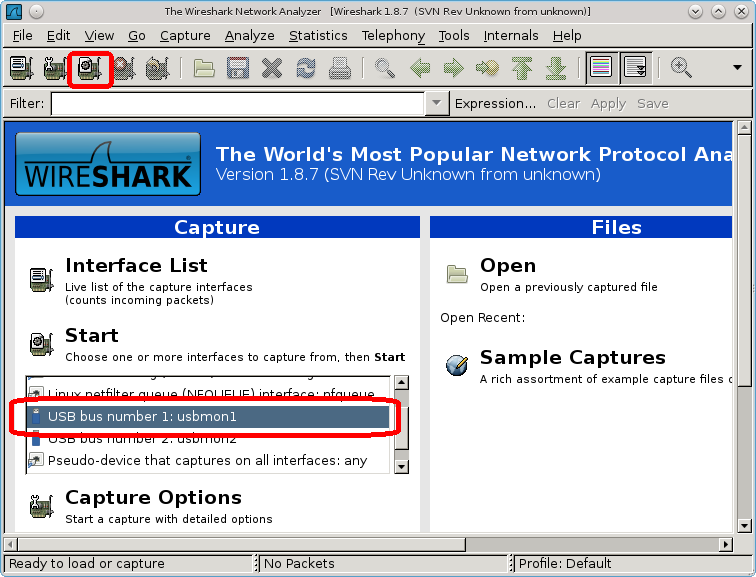
\includegraphics[width=10cm]{12_wireshark.png}
\end{figure}

Для анализа протокола нам необходимо перехватить следующие части генерируемого траффика:

\begin{itemize}
  \item инициализация устройства
  \item начало выполнения какой"=либо функции
  \item окончание выполнения какой"=либо функции
  \item деинициализация устройства
\end{itemize}

Обычно данные части отделены по времени, т.к. инициировать выполнения функции устройством можно в произвольное время (например, подвинуть мышку, нажать кнопку на клавиатуре, начать захват видео с веб"=камеры и т.д.)

Как правило, изучаемые устройства делятся на два типа:

\begin{itemize}
  \item Register"=oriented устройства
  \item Message"=oriented устройства
\end{itemize}

Для первых в перехватываемых трансферах будет чётко прослеживаться следующая структура:

\begin{itemize}
  \item заголовок трансфера (например, размер в байтах)
  \item адрес регистра
  \item значение (несколько значений)
  \item хвост трансфера (например, контрольная сумма)
\end{itemize}

Данные устройства предоставляют некое адресное пространство, в которое мы можем производить запись/чтение с помощью определённых USB"=трансферов.

Пример данного трансфера мы видим на иллюстрации:

\begin{figure}[h!]
  \centering
  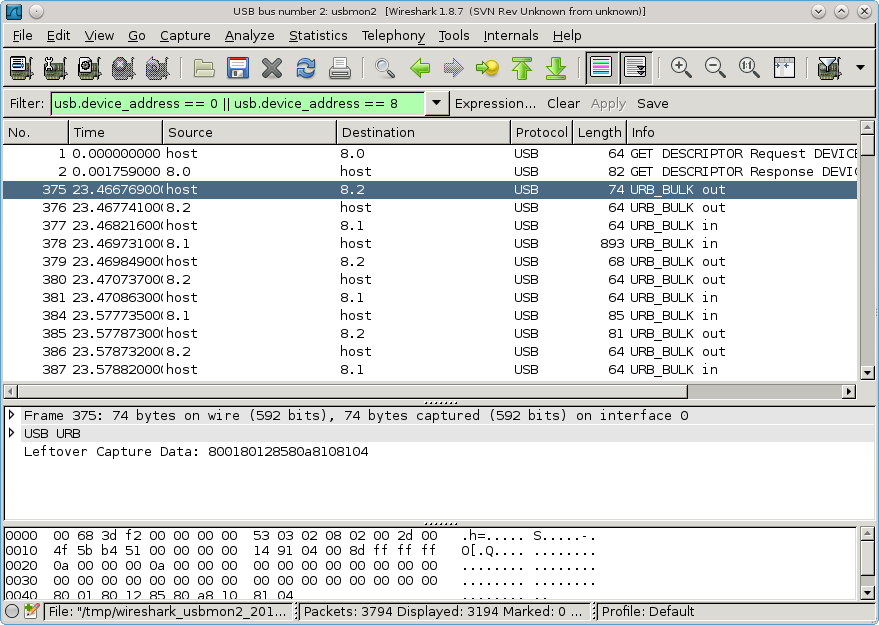
\includegraphics[width=10cm]{12_traffic-sample.png}
\end{figure}

См. трансфер \No 375, поле leftover capture data. В данном случае трансфер содержит пары адрес"=регистра "--- значение. Трансфер №376 является подтверждением, что устройство приняло трансфер. Трансфер \No 377 является запросом от хоста на приём данных от устройства, трансфер №378 "--- ответом устройства. Можно заметить, что любой трансфер в Wireshark виден как пара пакетов вида запрос хоста "--- ответ устройства (надеюсь, читатель еще помнить что все трансферы на USB шине инициирует хост?). Стоит отметить, что не всегда эта пара расположена линейно.

Для второго типа устройств в перехватываемых трансферах будет видна следующая структура:

\begin{itemize}
  \item заголовок трансфера
  \item тип сообщения
  \item тело сообщения
  \item хвост трансфера
\end{itemize}

Данные устройства, как правило, требуют больших усилий по расшифровке протокола.

Как правило, практически невозможно по дампу траффика, без экспериментов с устройством, расшифровать протокол. Для экспериментов удобно будет написать прототип драйвера с использованием библиотеки libusb. Данная библиотека работает в пространстве пользователя, т.о. при падении Вашего прототипа не упадёт вся ОС.

В качестве первого прототипа разумно будет повторить ту последовательность, которая записана в дампе. При запуске прототипа стоит записать еще один дамп, и сравнить его с оригинальным. Отличия между дампами сигнализируют о том, что что"=то прототип делает не так. Модификациями прототипа необходимо добиться идентичности дампа (в некоторых случаях это необязательно или невозможно, например при захвате картинки с камеры).

Пример простейших прототипов можно посмотреть в \cite{Anar4} и \cite{Anar5}. Как можно заметить данные прототипы состоят из следующих частей:

\begin{itemize}
  \item инициализация библиотеки: libusb\_init()
  \item открытие устройства: libusb\_open\_device\_with\_vid\_pid()
  \item выбор нужного интерфейса:  libusb\_claim\_interface()
  \item некоторого количества трансферов: libusb\_bulk\_transfer()/libusb\_control\_transfer()/libusb\_interrupt\_transfer()
  \item разбор ответа от устройства
  \item деинициализация: libusb\_close(); libusb\_exit()
\end{itemize}

\subsection*{Заключение}

Не смотря на то, что разбор протокола USB"=устройства кажется сложной задачей, на самом деле таковым не является "--- необходимо лишь упорство, терпение и желание экспериментировать.

\begin{thebibliography}{9}
\bibitem{Anar1} \url{http://www.beyondlogic.org/usbnutshell/usb1.shtml}
\bibitem{Anar2} \url{https://www.kernel.org/doc/Documentation/usb/usbmon.txt}
\bibitem{Anar3} \url{http://desowin.org/usbpcap/}
\bibitem{Anar4} \url{https://github.com/anarsoul/fprint\_aes1660}
\bibitem{Anar5} \url{https://github.com/anarsoul/fprint\_aes2550}
\end{thebibliography}

\end{document}




